\documentclass[]{article}
\usepackage{lmodern}
\usepackage{amssymb,amsmath}
\usepackage{ifxetex,ifluatex}
\usepackage{fixltx2e} % provides \textsubscript
\ifnum 0\ifxetex 1\fi\ifluatex 1\fi=0 % if pdftex
  \usepackage[T1]{fontenc}
  \usepackage[utf8]{inputenc}
\else % if luatex or xelatex
  \ifxetex
    \usepackage{mathspec}
  \else
    \usepackage{fontspec}
  \fi
  \defaultfontfeatures{Ligatures=TeX,Scale=MatchLowercase}
\fi
% use upquote if available, for straight quotes in verbatim environments
\IfFileExists{upquote.sty}{\usepackage{upquote}}{}
% use microtype if available
\IfFileExists{microtype.sty}{%
\usepackage{microtype}
\UseMicrotypeSet[protrusion]{basicmath} % disable protrusion for tt fonts
}{}
\usepackage[margin=2.54cm]{geometry}
\usepackage{hyperref}
\hypersetup{unicode=true,
            pdftitle={11: Generalized Linear Models},
            pdfauthor={Environmental Data Analytics \textbar{} Kateri Salk},
            pdfborder={0 0 0},
            breaklinks=true}
\urlstyle{same}  % don't use monospace font for urls
\usepackage{color}
\usepackage{fancyvrb}
\newcommand{\VerbBar}{|}
\newcommand{\VERB}{\Verb[commandchars=\\\{\}]}
\DefineVerbatimEnvironment{Highlighting}{Verbatim}{commandchars=\\\{\}}
% Add ',fontsize=\small' for more characters per line
\usepackage{framed}
\definecolor{shadecolor}{RGB}{248,248,248}
\newenvironment{Shaded}{\begin{snugshade}}{\end{snugshade}}
\newcommand{\KeywordTok}[1]{\textcolor[rgb]{0.13,0.29,0.53}{\textbf{#1}}}
\newcommand{\DataTypeTok}[1]{\textcolor[rgb]{0.13,0.29,0.53}{#1}}
\newcommand{\DecValTok}[1]{\textcolor[rgb]{0.00,0.00,0.81}{#1}}
\newcommand{\BaseNTok}[1]{\textcolor[rgb]{0.00,0.00,0.81}{#1}}
\newcommand{\FloatTok}[1]{\textcolor[rgb]{0.00,0.00,0.81}{#1}}
\newcommand{\ConstantTok}[1]{\textcolor[rgb]{0.00,0.00,0.00}{#1}}
\newcommand{\CharTok}[1]{\textcolor[rgb]{0.31,0.60,0.02}{#1}}
\newcommand{\SpecialCharTok}[1]{\textcolor[rgb]{0.00,0.00,0.00}{#1}}
\newcommand{\StringTok}[1]{\textcolor[rgb]{0.31,0.60,0.02}{#1}}
\newcommand{\VerbatimStringTok}[1]{\textcolor[rgb]{0.31,0.60,0.02}{#1}}
\newcommand{\SpecialStringTok}[1]{\textcolor[rgb]{0.31,0.60,0.02}{#1}}
\newcommand{\ImportTok}[1]{#1}
\newcommand{\CommentTok}[1]{\textcolor[rgb]{0.56,0.35,0.01}{\textit{#1}}}
\newcommand{\DocumentationTok}[1]{\textcolor[rgb]{0.56,0.35,0.01}{\textbf{\textit{#1}}}}
\newcommand{\AnnotationTok}[1]{\textcolor[rgb]{0.56,0.35,0.01}{\textbf{\textit{#1}}}}
\newcommand{\CommentVarTok}[1]{\textcolor[rgb]{0.56,0.35,0.01}{\textbf{\textit{#1}}}}
\newcommand{\OtherTok}[1]{\textcolor[rgb]{0.56,0.35,0.01}{#1}}
\newcommand{\FunctionTok}[1]{\textcolor[rgb]{0.00,0.00,0.00}{#1}}
\newcommand{\VariableTok}[1]{\textcolor[rgb]{0.00,0.00,0.00}{#1}}
\newcommand{\ControlFlowTok}[1]{\textcolor[rgb]{0.13,0.29,0.53}{\textbf{#1}}}
\newcommand{\OperatorTok}[1]{\textcolor[rgb]{0.81,0.36,0.00}{\textbf{#1}}}
\newcommand{\BuiltInTok}[1]{#1}
\newcommand{\ExtensionTok}[1]{#1}
\newcommand{\PreprocessorTok}[1]{\textcolor[rgb]{0.56,0.35,0.01}{\textit{#1}}}
\newcommand{\AttributeTok}[1]{\textcolor[rgb]{0.77,0.63,0.00}{#1}}
\newcommand{\RegionMarkerTok}[1]{#1}
\newcommand{\InformationTok}[1]{\textcolor[rgb]{0.56,0.35,0.01}{\textbf{\textit{#1}}}}
\newcommand{\WarningTok}[1]{\textcolor[rgb]{0.56,0.35,0.01}{\textbf{\textit{#1}}}}
\newcommand{\AlertTok}[1]{\textcolor[rgb]{0.94,0.16,0.16}{#1}}
\newcommand{\ErrorTok}[1]{\textcolor[rgb]{0.64,0.00,0.00}{\textbf{#1}}}
\newcommand{\NormalTok}[1]{#1}
\usepackage{graphicx,grffile}
\makeatletter
\def\maxwidth{\ifdim\Gin@nat@width>\linewidth\linewidth\else\Gin@nat@width\fi}
\def\maxheight{\ifdim\Gin@nat@height>\textheight\textheight\else\Gin@nat@height\fi}
\makeatother
% Scale images if necessary, so that they will not overflow the page
% margins by default, and it is still possible to overwrite the defaults
% using explicit options in \includegraphics[width, height, ...]{}
\setkeys{Gin}{width=\maxwidth,height=\maxheight,keepaspectratio}
\IfFileExists{parskip.sty}{%
\usepackage{parskip}
}{% else
\setlength{\parindent}{0pt}
\setlength{\parskip}{6pt plus 2pt minus 1pt}
}
\setlength{\emergencystretch}{3em}  % prevent overfull lines
\providecommand{\tightlist}{%
  \setlength{\itemsep}{0pt}\setlength{\parskip}{0pt}}
\setcounter{secnumdepth}{0}
% Redefines (sub)paragraphs to behave more like sections
\ifx\paragraph\undefined\else
\let\oldparagraph\paragraph
\renewcommand{\paragraph}[1]{\oldparagraph{#1}\mbox{}}
\fi
\ifx\subparagraph\undefined\else
\let\oldsubparagraph\subparagraph
\renewcommand{\subparagraph}[1]{\oldsubparagraph{#1}\mbox{}}
\fi

%%% Use protect on footnotes to avoid problems with footnotes in titles
\let\rmarkdownfootnote\footnote%
\def\footnote{\protect\rmarkdownfootnote}

%%% Change title format to be more compact
\usepackage{titling}

% Create subtitle command for use in maketitle
\newcommand{\subtitle}[1]{
  \posttitle{
    \begin{center}\large#1\end{center}
    }
}

\setlength{\droptitle}{-2em}

  \title{11: Generalized Linear Models}
    \pretitle{\vspace{\droptitle}\centering\huge}
  \posttitle{\par}
    \author{Environmental Data Analytics \textbar{} Kateri Salk}
    \preauthor{\centering\large\emph}
  \postauthor{\par}
      \predate{\centering\large\emph}
  \postdate{\par}
    \date{Spring 2019}


\begin{document}
\maketitle

\subsection{LESSON OBJECTIVES}\label{lesson-objectives}

\begin{enumerate}
\def\labelenumi{\arabic{enumi}.}
\tightlist
\item
  Describe the components of the generalized linear model (GLM)
\item
  Apply special cases of the GLM to real datasets
\item
  Interpret and report the results of GLMs in publication-style formats
\end{enumerate}

\subsection{SET UP YOUR DATA ANALYSIS
SESSION}\label{set-up-your-data-analysis-session}

\begin{Shaded}
\begin{Highlighting}[]
\KeywordTok{getwd}\NormalTok{()}
\end{Highlighting}
\end{Shaded}

\begin{verbatim}
## [1] "C:/Users/Felipe/OneDrive - Duke University/1. DUKE/1. Ramos 2 Semestre/EOS-872 Env. Data Analytics/Environmental_Data_Analytics"
\end{verbatim}

\begin{Shaded}
\begin{Highlighting}[]
\KeywordTok{library}\NormalTok{(tidyverse)}

\NormalTok{PeterPaul.nutrients <-}\StringTok{ }\KeywordTok{read.csv}\NormalTok{(}\StringTok{"./Data/Processed/NTL-LTER_Lake_Nutrients_PeterPaul_Processed.csv"}\NormalTok{)}
\NormalTok{EPAair <-}\StringTok{ }\KeywordTok{read.csv}\NormalTok{(}\StringTok{"./Data/Processed/EPAair_O3PM25_3sites1718_processed.csv"}\NormalTok{)}

\CommentTok{# Set date to date format}
\NormalTok{EPAair}\OperatorTok{$}\NormalTok{Date <-}\StringTok{ }\KeywordTok{as.Date}\NormalTok{(EPAair}\OperatorTok{$}\NormalTok{Date, }\DataTypeTok{format =} \StringTok{"%Y-%m-%d"}\NormalTok{)}
\NormalTok{PeterPaul.nutrients}\OperatorTok{$}\NormalTok{sampledate <-}\StringTok{ }\KeywordTok{as.Date}\NormalTok{(PeterPaul.nutrients}\OperatorTok{$}\NormalTok{sampledate, }\DataTypeTok{format =} \StringTok{"%Y-%m-%d"}\NormalTok{)}

\CommentTok{# remove negative values for depth_id}
\NormalTok{PeterPaul.nutrients <-}\StringTok{ }\KeywordTok{filter}\NormalTok{(PeterPaul.nutrients, depth_id }\OperatorTok{>}\StringTok{ }\DecValTok{0}\NormalTok{) }\CommentTok{#is a weird ID that was given. Just remove for this example. }

\CommentTok{# set depth_id to factor}
\NormalTok{PeterPaul.nutrients}\OperatorTok{$}\NormalTok{depth_id <-}\StringTok{ }\KeywordTok{as.factor}\NormalTok{(PeterPaul.nutrients}\OperatorTok{$}\NormalTok{depth_id) }\CommentTok{# we want later factor instead of numeric.}

\NormalTok{mytheme <-}\StringTok{ }\KeywordTok{theme_classic}\NormalTok{(}\DataTypeTok{base_size =} \DecValTok{14}\NormalTok{) }\OperatorTok{+}
\StringTok{  }\KeywordTok{theme}\NormalTok{(}\DataTypeTok{axis.text =} \KeywordTok{element_text}\NormalTok{(}\DataTypeTok{color =} \StringTok{"black"}\NormalTok{), }
        \DataTypeTok{legend.position =} \StringTok{"top"}\NormalTok{)}
\KeywordTok{theme_set}\NormalTok{(mytheme)}
\end{Highlighting}
\end{Shaded}

\subsection{GENERALIZED LINEAR MODELS}\label{generalized-linear-models}

The one-sample test (model of the mean), two-sample t-test, analysis of
variance (ANOVA), and linear regression are all special cases of the
\textbf{generalized linear model} (GLM). The GLM also includes analyses
not covered in this class, including logistic regression, multinomial
regression, chi square, and log-linear models. The common characteristic
of general linear models is the expression of a continuous response
variable as a linear combination of the effects of categorical or
continuous explanatory variables, plus an error term that expresses the
random error associated with the coefficients of all explanatory
variables. The explanatory variables comprise the deterministic
component of the model, and the error term comprises the stochastic
component of the model. Historically, artificial distinctions were made
between linear models that contained categorical and continuous
explanatory variables, but this distinction is no longer made. The
inclusion of these models within the umbrella of the GLM allows models
to fit the main effects of both categorical and continuous explanatory
variables as well as their interactions.

\subsubsection{\texorpdfstring{Choosing a model from your data: A
``cheat
sheet''}{Choosing a model from your data: A cheat sheet}}\label{choosing-a-model-from-your-data-a-cheat-sheet}

\textbf{T-test:} Continuous response, one categorical explanatory
variable with two categories (or comparison to a single value if a
one-sample test).

\textbf{One-way ANOVA (Analysis of Variance):} Continuous response, one
categorical explanatory variable with more than two categories.

\textbf{Two-way ANOVA (Analysis of Variance)} Continuous response, two
categorical explanatory variables.

\textbf{Single Linear Regression} Continuous response, one continuous
explanatory variable.

\textbf{Multiple Linear Regression} Continuous response, two or more
continuous explanatory variables.

\textbf{ANCOVA (Analysis of Covariance)} Continuous response,
categorical explanatory variable(s) and continuous explanatory
variable(s).

If multiple explanatory variables are chosen, they may be analyzed with
respect to their \textbf{main effects} on the model (i.e., their
separate impacts on the variance explained) or with respsect to their
\textbf{interaction effects,} the effect of interacting explanatory
variables on the model.

\subsubsection{Assumptions of the GLM}\label{assumptions-of-the-glm}

The GLM is based on the assumption that the data approximate a normal
distribution (or a linearly transformed normal distribution). We will
discuss the non-parametric analogues to several of these tests if the
assumptions of normality are violated. For tests that analyze
categorical explanatory variables, the assumption is that the variance
in the response variable is equal among groups. Note: environmental data
often violate the assumptions of normality and equal variance, and we
will often proceed with a GLM even if these assumptions are violated. In
this situation, you must justify your decision.

\subsection{T-TEST AND ONE-WAY ANOVA}\label{t-test-and-one-way-anova}

\subsubsection{One-sample t-test}\label{one-sample-t-test}

The object of a one sample test is to test the null hypothesis that the
mean of the group is equal to a specific value. For example, we might
ask ourselves (from the EPA air quality processed dataset):

Are Ozone levels below the threshold for ``good'' AQI index (0-50)? \#T
test.

\begin{Shaded}
\begin{Highlighting}[]
\KeywordTok{summary}\NormalTok{(EPAair}\OperatorTok{$}\NormalTok{Ozone)}
\end{Highlighting}
\end{Shaded}

\begin{verbatim}
##    Min. 1st Qu.  Median    Mean 3rd Qu.    Max.    NA's 
##    5.00   31.00   37.00   36.92   44.00   97.00     868
\end{verbatim}

\begin{Shaded}
\begin{Highlighting}[]
\CommentTok{# Evaluate assumption of normal distribution}
\KeywordTok{shapiro.test}\NormalTok{(EPAair}\OperatorTok{$}\NormalTok{Ozone) }\CommentTok{#test aprox. to normal dist. pvalue less than 5% not Ok. So lets take a look}
\end{Highlighting}
\end{Shaded}

\begin{verbatim}
## 
##  Shapiro-Wilk normality test
## 
## data:  EPAair$Ozone
## W = 0.97317, p-value = 2.747e-13
\end{verbatim}

\begin{Shaded}
\begin{Highlighting}[]
\KeywordTok{ggplot}\NormalTok{(EPAair, }\KeywordTok{aes}\NormalTok{(}\DataTypeTok{x =}\NormalTok{ Ozone)) }\OperatorTok{+}
\StringTok{  }\KeywordTok{geom_histogram}\NormalTok{(}\DataTypeTok{stat =} \StringTok{"count"}\NormalTok{) }\CommentTok{#wrong peak and long tail to the right}
\end{Highlighting}
\end{Shaded}

\begin{verbatim}
## Warning: Ignoring unknown parameters: binwidth, bins, pad
\end{verbatim}

\begin{verbatim}
## Warning: Removed 868 rows containing non-finite values (stat_count).
\end{verbatim}

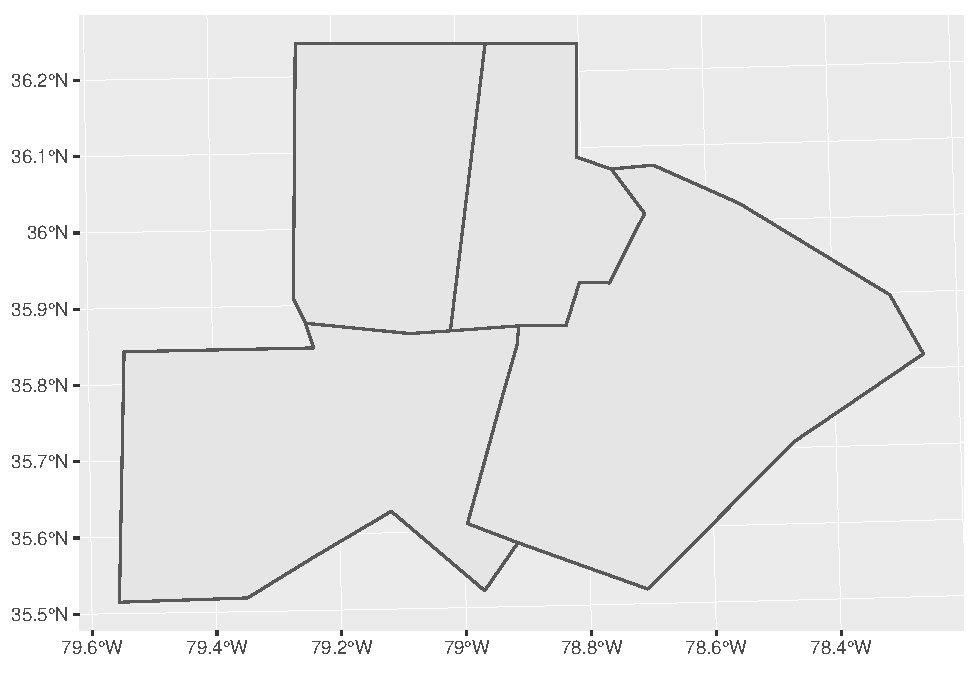
\includegraphics{11_GLMs_files/figure-latex/unnamed-chunk-2-1.pdf}

\begin{Shaded}
\begin{Highlighting}[]
\KeywordTok{qqnorm}\NormalTok{(EPAair}\OperatorTok{$}\NormalTok{Ozone); }\KeywordTok{qqline}\NormalTok{(EPAair}\OperatorTok{$}\NormalTok{Ozone) }\CommentTok{# other way to look at it. We go ahead any way becuase a lot of data and shape resembles}
\end{Highlighting}
\end{Shaded}

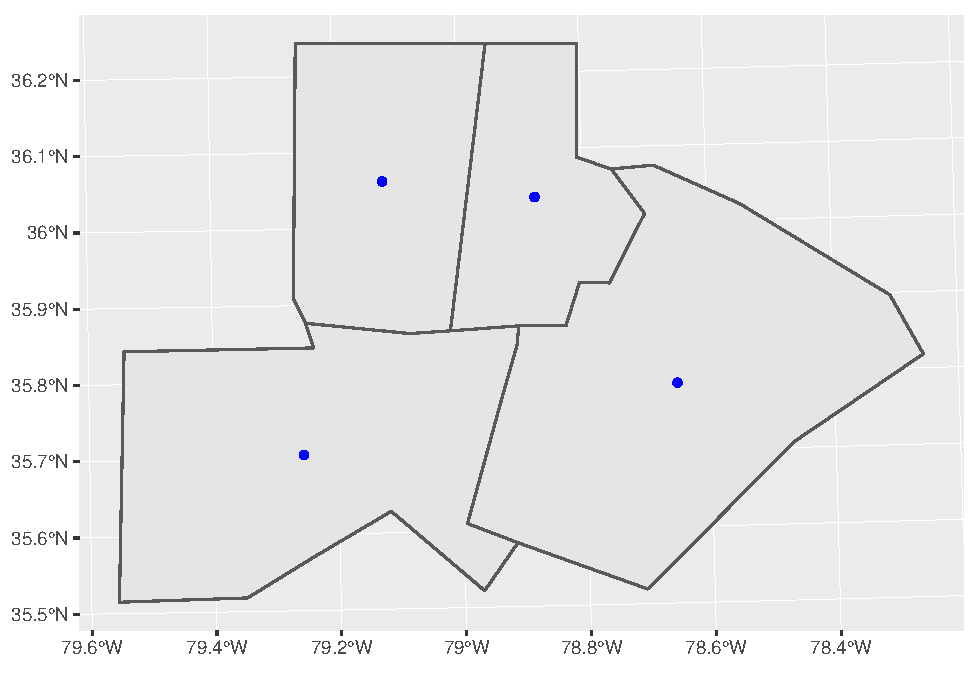
\includegraphics{11_GLMs_files/figure-latex/unnamed-chunk-2-2.pdf}

\begin{Shaded}
\begin{Highlighting}[]
\NormalTok{O3.onesample <-}\StringTok{ }\KeywordTok{t.test}\NormalTok{(EPAair}\OperatorTok{$}\NormalTok{Ozone, }\DataTypeTok{mu =} \DecValTok{50}\NormalTok{, }\DataTypeTok{alternative =} \StringTok{"less"}\NormalTok{) }\CommentTok{# we are asking if data below threshold than 50.}
\NormalTok{O3.onesample }\CommentTok{# store the result. P value low. reject null hypothesis. give also t score. Linear model y = 36.9 ] error}
\end{Highlighting}
\end{Shaded}

\begin{verbatim}
## 
##  One Sample t-test
## 
## data:  EPAair$Ozone
## t = -41.911, df = 1084, p-value < 2.2e-16
## alternative hypothesis: true mean is less than 50
## 95 percent confidence interval:
##      -Inf 37.43006
## sample estimates:
## mean of x 
##  36.91613
\end{verbatim}

What information does the output give us? How might we report this
information in a report?

\begin{quote}
ANSWER: Ozone AQI values in 2017-2018 were significanly lower than 50
(one sample t-test; t = -41.9, df =184, p\textless{}0.0001)
\end{quote}

\subsubsection{Two-sample t-test \#second alpha value in the linear
model}\label{two-sample-t-test-second-alpha-value-in-the-linear-model}

The two-sample \emph{t} test is used to test the hypothesis that the
mean of two samples is equivalent. Unlike the one-sample tests, a
two-sample test requires a second assumption that the variance of the
two groups is equivalent. Are Ozone levels different between Blackstone
and Bryson City?

\begin{Shaded}
\begin{Highlighting}[]
\KeywordTok{shapiro.test}\NormalTok{(EPAair}\OperatorTok{$}\NormalTok{Ozone[EPAair}\OperatorTok{$}\NormalTok{Site.Name }\OperatorTok{==}\StringTok{ "Blackstone"}\NormalTok{])}
\end{Highlighting}
\end{Shaded}

\begin{verbatim}
## 
##  Shapiro-Wilk normality test
## 
## data:  EPAair$Ozone[EPAair$Site.Name == "Blackstone"]
## W = 0.97221, p-value = 6.349e-09
\end{verbatim}

\begin{Shaded}
\begin{Highlighting}[]
\KeywordTok{shapiro.test}\NormalTok{(EPAair}\OperatorTok{$}\NormalTok{Ozone[EPAair}\OperatorTok{$}\NormalTok{Site.Name }\OperatorTok{==}\StringTok{ "Bryson City"}\NormalTok{])}
\end{Highlighting}
\end{Shaded}

\begin{verbatim}
## 
##  Shapiro-Wilk normality test
## 
## data:  EPAair$Ozone[EPAair$Site.Name == "Bryson City"]
## W = 0.97189, p-value = 2.228e-08
\end{verbatim}

\begin{Shaded}
\begin{Highlighting}[]
\KeywordTok{var.test}\NormalTok{(EPAair}\OperatorTok{$}\NormalTok{Ozone }\OperatorTok{~}\StringTok{ }\NormalTok{EPAair}\OperatorTok{$}\NormalTok{Site.Name) }\CommentTok{# f statistic and pvalue. variance the same? Pvalue low, the variance is not the same. The interval does not overlap 1.}
\end{Highlighting}
\end{Shaded}

\begin{verbatim}
## 
##  F test to compare two variances
## 
## data:  EPAair$Ozone by EPAair$Site.Name
## F = 1.3678, num df = 569, denom df = 514, p-value = 0.0002955
## alternative hypothesis: true ratio of variances is not equal to 1
## 95 percent confidence interval:
##  1.154854 1.618780
## sample estimates:
## ratio of variances 
##           1.367782
\end{verbatim}

\begin{Shaded}
\begin{Highlighting}[]
\KeywordTok{ggplot}\NormalTok{(EPAair, }\KeywordTok{aes}\NormalTok{(}\DataTypeTok{x =}\NormalTok{ Ozone, }\DataTypeTok{color =}\NormalTok{ Site.Name)) }\OperatorTok{+}
\StringTok{  }\KeywordTok{geom_freqpoly}\NormalTok{(}\DataTypeTok{stat =} \StringTok{"count"}\NormalTok{) }\CommentTok{# just to look how they relate to each other (look at tails, peaks)}
\end{Highlighting}
\end{Shaded}

\begin{verbatim}
## Warning: Removed 868 rows containing non-finite values (stat_count).
\end{verbatim}

\includegraphics{11_GLMs_files/figure-latex/unnamed-chunk-3-1.pdf}

\begin{Shaded}
\begin{Highlighting}[]
\CommentTok{# two ways of doing it}
\CommentTok{# Format as a t-test}
\NormalTok{O3.twosample <-}\StringTok{ }\KeywordTok{t.test}\NormalTok{(EPAair}\OperatorTok{$}\NormalTok{Ozone }\OperatorTok{~}\StringTok{ }\NormalTok{EPAair}\OperatorTok{$}\NormalTok{Site.Name)}
\NormalTok{O3.twosample}
\end{Highlighting}
\end{Shaded}

\begin{verbatim}
## 
##  Welch Two Sample t-test
## 
## data:  EPAair$Ozone by EPAair$Site.Name
## t = 5.3875, df = 1079.8, p-value = 8.766e-08
## alternative hypothesis: true difference in means is not equal to 0
## 95 percent confidence interval:
##  2.098082 4.501782
## sample estimates:
##  mean in group Blackstone mean in group Bryson City 
##                  38.48246                  35.18252
\end{verbatim}

\begin{Shaded}
\begin{Highlighting}[]
\NormalTok{O3.twosample}\OperatorTok{$}\NormalTok{p.value }\CommentTok{# we have a significance differnet in the means between the 2 groups.}
\end{Highlighting}
\end{Shaded}

\begin{verbatim}
## [1] 8.765983e-08
\end{verbatim}

\begin{Shaded}
\begin{Highlighting}[]
\CommentTok{# so the linear model is y = Blackstone(38.48) + BrysonCity(35.18) + error}
\CommentTok{# Format as a GLM #other way of doing it}
\NormalTok{O3.twosample2 <-}\StringTok{ }\KeywordTok{lm}\NormalTok{(EPAair}\OperatorTok{$}\NormalTok{Ozone }\OperatorTok{~}\StringTok{ }\NormalTok{EPAair}\OperatorTok{$}\NormalTok{Site.Name)}
\KeywordTok{summary}\NormalTok{(O3.twosample2) }\CommentTok{#diff pvalue. same estimates but bryson is relative. We get a lot of aditional info not useful right now.}
\end{Highlighting}
\end{Shaded}

\begin{verbatim}
## 
## Call:
## lm(formula = EPAair$Ozone ~ EPAair$Site.Name)
## 
## Residuals:
##     Min      1Q  Median      3Q     Max 
## -30.482  -6.183  -0.183   5.518  58.518 
## 
## Coefficients:
##                             Estimate Std. Error t value Pr(>|t|)    
## (Intercept)                  38.4825     0.4253  90.477  < 2e-16 ***
## EPAair$Site.NameBryson City  -3.2999     0.6174  -5.345  1.1e-07 ***
## ---
## Signif. codes:  0 '***' 0.001 '**' 0.01 '*' 0.05 '.' 0.1 ' ' 1
## 
## Residual standard error: 10.15 on 1083 degrees of freedom
##   (868 observations deleted due to missingness)
## Multiple R-squared:  0.0257, Adjusted R-squared:  0.0248 
## F-statistic: 28.57 on 1 and 1083 DF,  p-value: 1.101e-07
\end{verbatim}

\subsubsection{Non-parametric equivalent of t-test: Wilcoxon test \#for
not normal distribution. distribution
free}\label{non-parametric-equivalent-of-t-test-wilcoxon-test-for-not-normal-distribution.-distribution-free}

When we wish to avoid the assumption of normality, we can apply
\emph{distribution-free}, or non-parametric, methods in the form of the
Wilcoxon rank sum (Mann-Whitney) test. The Wilcoxon test replaces the
data by their rank and calculates the sum of the ranks for each group.
Notice that the output of the Wilcoxon test is more limited than its
parametric equivalent.

\begin{Shaded}
\begin{Highlighting}[]
\NormalTok{O3.onesample.wilcox <-}\StringTok{ }\KeywordTok{wilcox.test}\NormalTok{(EPAair}\OperatorTok{$}\NormalTok{Ozone, }\DataTypeTok{mu =} \DecValTok{50}\NormalTok{, }\DataTypeTok{alternative =} \StringTok{"less"}\NormalTok{)}
\NormalTok{O3.onesample.wilcox}
\end{Highlighting}
\end{Shaded}

\begin{verbatim}
## 
##  Wilcoxon signed rank test with continuity correction
## 
## data:  EPAair$Ozone
## V = 25828, p-value < 2.2e-16
## alternative hypothesis: true location is less than 50
\end{verbatim}

\begin{Shaded}
\begin{Highlighting}[]
\NormalTok{O3.twosample.wilcox <-}\StringTok{ }\KeywordTok{wilcox.test}\NormalTok{(EPAair}\OperatorTok{$}\NormalTok{Ozone }\OperatorTok{~}\StringTok{ }\NormalTok{EPAair}\OperatorTok{$}\NormalTok{Site.Name)}
\NormalTok{O3.twosample.wilcox }\CommentTok{# much more limited models but we get the info that we wanted. dont tell us the prediction for the means. less explanatory power.}
\end{Highlighting}
\end{Shaded}

\begin{verbatim}
## 
##  Wilcoxon rank sum test with continuity correction
## 
## data:  EPAair$Ozone by EPAair$Site.Name
## W = 175960, p-value = 1.451e-08
## alternative hypothesis: true location shift is not equal to 0
\end{verbatim}

\subsubsection{One-way ANOVA}\label{one-way-anova}

A one-way ANOVA is the same test in practice as a two-sample t-test but
for three or more groups. In R, we can run the model with the function
\texttt{lm} or \texttt{aov}, the latter of which which will allow us to
run post-hoc tests to determine pairwise differences.

Are PM2.5 levels different between Blackstone, Bryson City, and Triple
Oak?

\begin{Shaded}
\begin{Highlighting}[]
\KeywordTok{shapiro.test}\NormalTok{(EPAair}\OperatorTok{$}\NormalTok{PM2.}\DecValTok{5}\NormalTok{[EPAair}\OperatorTok{$}\NormalTok{Site.Name }\OperatorTok{==}\StringTok{ "Blackstone"}\NormalTok{])}
\end{Highlighting}
\end{Shaded}

\begin{verbatim}
## 
##  Shapiro-Wilk normality test
## 
## data:  EPAair$PM2.5[EPAair$Site.Name == "Blackstone"]
## W = 0.99335, p-value = 0.01489
\end{verbatim}

\begin{Shaded}
\begin{Highlighting}[]
\KeywordTok{shapiro.test}\NormalTok{(EPAair}\OperatorTok{$}\NormalTok{PM2.}\DecValTok{5}\NormalTok{[EPAair}\OperatorTok{$}\NormalTok{Site.Name }\OperatorTok{==}\StringTok{ "Bryson City"}\NormalTok{])}
\end{Highlighting}
\end{Shaded}

\begin{verbatim}
## 
##  Shapiro-Wilk normality test
## 
## data:  EPAair$PM2.5[EPAair$Site.Name == "Bryson City"]
## W = 0.98207, p-value = 2.527e-07
\end{verbatim}

\begin{Shaded}
\begin{Highlighting}[]
\KeywordTok{shapiro.test}\NormalTok{(EPAair}\OperatorTok{$}\NormalTok{PM2.}\DecValTok{5}\NormalTok{[EPAair}\OperatorTok{$}\NormalTok{Site.Name }\OperatorTok{==}\StringTok{ "Triple Oak"}\NormalTok{])}
\end{Highlighting}
\end{Shaded}

\begin{verbatim}
## 
##  Shapiro-Wilk normality test
## 
## data:  EPAair$PM2.5[EPAair$Site.Name == "Triple Oak"]
## W = 0.99064, p-value = 0.0002744
\end{verbatim}

\begin{Shaded}
\begin{Highlighting}[]
\KeywordTok{ggplot}\NormalTok{(EPAair, }\KeywordTok{aes}\NormalTok{(}\DataTypeTok{x =}\NormalTok{ PM2.}\DecValTok{5}\NormalTok{, }\DataTypeTok{color =}\NormalTok{ Site.Name)) }\OperatorTok{+}
\StringTok{  }\KeywordTok{geom_freqpoly}\NormalTok{(}\DataTypeTok{stat =} \StringTok{"count"}\NormalTok{) }\CommentTok{# fairly good bell curve. not crazy tails. maybe we may wanna proceed with anova}
\end{Highlighting}
\end{Shaded}

\begin{verbatim}
## Warning: Removed 52 rows containing non-finite values (stat_count).
\end{verbatim}

\includegraphics{11_GLMs_files/figure-latex/unnamed-chunk-5-1.pdf}

\begin{Shaded}
\begin{Highlighting}[]
\KeywordTok{qqnorm}\NormalTok{(EPAair}\OperatorTok{$}\NormalTok{PM2.}\DecValTok{5}\NormalTok{); }\KeywordTok{qqline}\NormalTok{(EPAair}\OperatorTok{$}\NormalTok{PM2.}\DecValTok{5}\NormalTok{) }\CommentTok{# looks good except for the tails. not surprising for environ data.}
\end{Highlighting}
\end{Shaded}

\includegraphics{11_GLMs_files/figure-latex/unnamed-chunk-5-2.pdf}

\begin{Shaded}
\begin{Highlighting}[]
\KeywordTok{bartlett.test}\NormalTok{(EPAair}\OperatorTok{$}\NormalTok{PM2.}\DecValTok{5} \OperatorTok{~}\StringTok{ }\NormalTok{EPAair}\OperatorTok{$}\NormalTok{Site.Name) }\CommentTok{# var equal? here they are not significance diff. reach assumption of equal differnece.}
\end{Highlighting}
\end{Shaded}

\begin{verbatim}
## 
##  Bartlett test of homogeneity of variances
## 
## data:  EPAair$PM2.5 by EPAair$Site.Name
## Bartlett's K-squared = 4.9951, df = 2, p-value = 0.08229
\end{verbatim}

\begin{Shaded}
\begin{Highlighting}[]
\CommentTok{#two ways}
\CommentTok{# Format as a GLM}
\NormalTok{PM2.}\FloatTok{5.}\NormalTok{anova <-}\StringTok{ }\KeywordTok{lm}\NormalTok{(EPAair}\OperatorTok{$}\NormalTok{PM2.}\DecValTok{5} \OperatorTok{~}\StringTok{ }\NormalTok{EPAair}\OperatorTok{$}\NormalTok{Site.Name)}
\KeywordTok{summary}\NormalTok{(PM2.}\FloatTok{5.}\NormalTok{anova) }\CommentTok{# linear model y = 36.7261 - 4.4266Bryson -3.24TripleOak #here we only know that the intercept is signif diff from 0, and the other variables signif diff from intercept.}
\end{Highlighting}
\end{Shaded}

\begin{verbatim}
## 
## Call:
## lm(formula = EPAair$PM2.5 ~ EPAair$Site.Name)
## 
## Residuals:
##     Min      1Q  Median      3Q     Max 
## -36.726 -10.300  -0.726  10.274  46.274 
## 
## Coefficients:
##                             Estimate Std. Error t value Pr(>|t|)    
## (Intercept)                  36.7261     0.5902  62.231  < 2e-16 ***
## EPAair$Site.NameBryson City  -4.4266     0.7977  -5.549 3.28e-08 ***
## EPAair$Site.NameTriple Oak   -3.2461     0.7967  -4.075 4.80e-05 ***
## ---
## Signif. codes:  0 '***' 0.001 '**' 0.01 '*' 0.05 '.' 0.1 ' ' 1
## 
## Residual standard error: 13.9 on 1898 degrees of freedom
##   (52 observations deleted due to missingness)
## Multiple R-squared:  0.01674,    Adjusted R-squared:  0.01571 
## F-statistic: 16.16 on 2 and 1898 DF,  p-value: 1.1e-07
\end{verbatim}

\begin{Shaded}
\begin{Highlighting}[]
\CommentTok{# Format as an aov}
\NormalTok{PM2.}\FloatTok{5.}\NormalTok{anova2 <-}\StringTok{ }\KeywordTok{aov}\NormalTok{(EPAair}\OperatorTok{$}\NormalTok{PM2.}\DecValTok{5} \OperatorTok{~}\StringTok{ }\NormalTok{EPAair}\OperatorTok{$}\NormalTok{Site.Name)}
\KeywordTok{summary}\NormalTok{(PM2.}\FloatTok{5.}\NormalTok{anova2) }\CommentTok{#just give us if site is significant predictor. we need a posthoc test}
\end{Highlighting}
\end{Shaded}

\begin{verbatim}
##                    Df Sum Sq Mean Sq F value  Pr(>F)    
## EPAair$Site.Name    2   6247  3123.6   16.16 1.1e-07 ***
## Residuals        1898 366884   193.3                    
## ---
## Signif. codes:  0 '***' 0.001 '**' 0.01 '*' 0.05 '.' 0.1 ' ' 1
## 52 observations deleted due to missingness
\end{verbatim}

\begin{Shaded}
\begin{Highlighting}[]
\CommentTok{# Run a post-hoc test for pairwise differences}
\KeywordTok{TukeyHSD}\NormalTok{(PM2.}\FloatTok{5.}\NormalTok{anova2) }\CommentTok{#there is no diff between Triple and Bryson}
\end{Highlighting}
\end{Shaded}

\begin{verbatim}
##   Tukey multiple comparisons of means
##     95% family-wise confidence level
## 
## Fit: aov(formula = EPAair$PM2.5 ~ EPAair$Site.Name)
## 
## $`EPAair$Site.Name`
##                             diff        lwr       upr     p adj
## Bryson City-Blackstone -4.426573 -6.2976740 -2.555472 0.0000001
## Triple Oak-Blackstone  -3.246126 -5.1147155 -1.377537 0.0001419
## Triple Oak-Bryson City  1.180447 -0.5972964  2.958191 0.2645306
\end{verbatim}

\begin{Shaded}
\begin{Highlighting}[]
\CommentTok{# Plot the results}
\CommentTok{# How might you edit this graph to make it attractive?}
\CommentTok{# How might you illustrate significant differences?}
\NormalTok{PM2.}\FloatTok{5.}\NormalTok{anova.plot <-}\StringTok{ }\KeywordTok{ggplot}\NormalTok{(EPAair, }\KeywordTok{aes}\NormalTok{(}\DataTypeTok{x =}\NormalTok{ Site.Name, }\DataTypeTok{y =}\NormalTok{ PM2.}\DecValTok{5}\NormalTok{)) }\OperatorTok{+}
\StringTok{  }\KeywordTok{geom_violin}\NormalTok{(}\DataTypeTok{draw_quantiles =} \FloatTok{0.5}\NormalTok{)}
\KeywordTok{print}\NormalTok{(PM2.}\FloatTok{5.}\NormalTok{anova.plot) }\CommentTok{#to look at the distribution}
\end{Highlighting}
\end{Shaded}

\begin{verbatim}
## Warning: Removed 52 rows containing non-finite values (stat_ydensity).
\end{verbatim}

\includegraphics{11_GLMs_files/figure-latex/unnamed-chunk-5-3.pdf} What
information does the output give us? How might we report this
information in a report?

\begin{quote}
ANSWer: (ANOVA; F = 16.16, df =1898, p \textless{} 0.0001). Our average
pm25 values where signif\ldots{}. .On the plot. Put a star on blackstone
or group them (bryson and triple under a hay or something geomtext or
something)
\end{quote}

\subsubsection{Non-parametric equivalent of ANOVA: Kruskal-Wallis
Test}\label{non-parametric-equivalent-of-anova-kruskal-wallis-test}

As with the Wilcoxon test, the Kruskal-Wallis test is the non-parametric
counterpart to the one-way ANOVA. Here, the data from two or more
independent samples are replaced with their ranks without regard to the
grouping AND based on the between-group sum of squares calculations.

For multiple comparisons, a p-value \textless{} 0.05 indicates that
there is a significant difference between groups, but it does not
indicate which groups, or in this case, months, differ from each other.

To analyze specific pairs in the data, you must use a \emph{post hoc}
test. These include the Dunn's test, a pairwise Mann-Whitney with the
Bonferroni correction, or the Conover-Iman test.

\begin{Shaded}
\begin{Highlighting}[]
\NormalTok{PM2.}\FloatTok{5.}\NormalTok{kw <-}\StringTok{ }\KeywordTok{kruskal.test}\NormalTok{(EPAair}\OperatorTok{$}\NormalTok{PM2.}\DecValTok{5} \OperatorTok{~}\StringTok{ }\NormalTok{EPAair}\OperatorTok{$}\NormalTok{Site.Name)}
\NormalTok{PM2.}\FloatTok{5.}\NormalTok{kw }\CommentTok{# doesnt indicate which groups are diff.}
\end{Highlighting}
\end{Shaded}

\begin{verbatim}
## 
##  Kruskal-Wallis rank sum test
## 
## data:  EPAair$PM2.5 by EPAair$Site.Name
## Kruskal-Wallis chi-squared = 34.737, df = 2, p-value = 2.864e-08
\end{verbatim}

\begin{Shaded}
\begin{Highlighting}[]
\CommentTok{#the next tells you but we are not going to do it.}
\CommentTok{# There are two functions to run the Dunn Test}
\CommentTok{# dunn.test(EPAair$PM2.5, EPAair$Site.Name, kw = T, }
\CommentTok{#           table = F, list = T, method = "holm", altp = T)   #From package dunn.test}
\CommentTok{# dunnTest(EPAair$PM2.5, EPAair$Site.Name)                    #From package FSA}
\end{Highlighting}
\end{Shaded}

\subsection{TWO-WAY ANOVA \#convination of multiple diff outputs y =
alphaa1 + alphaa2+ alphab1 + alphab2 +
error}\label{two-way-anova-convination-of-multiple-diff-outputs-y-alphaa1-alphaa2-alphab1-alphab2-error}

\subsubsection{Main effects}\label{main-effects}

A two-way ANOVA allows us to examine the effects of two categorical
explanatory variables on a continuous response variable. Let's look at
the NTL-LTER nutrient dataset for Peter and Paul lakes. What if we
wanted to know if total nitrogen concentrations differed based on lake
and depth?

\begin{Shaded}
\begin{Highlighting}[]
\NormalTok{TNanova.main <-}\StringTok{ }\KeywordTok{lm}\NormalTok{(PeterPaul.nutrients}\OperatorTok{$}\NormalTok{tn_ug }\OperatorTok{~}\StringTok{ }\NormalTok{PeterPaul.nutrients}\OperatorTok{$}\NormalTok{lakename }\OperatorTok{+}\StringTok{ }\CommentTok{# the plus is the main effefct anova}
\StringTok{                     }\NormalTok{PeterPaul.nutrients}\OperatorTok{$}\NormalTok{depth_id)}
\KeywordTok{summary}\NormalTok{(TNanova.main) }\CommentTok{#TN = y = 309(paul lake dpeth id of 1) + 105.2PeterLake(id1) + 97id2.. + error. id5 and id6 dont have relevant pvalues.}
\end{Highlighting}
\end{Shaded}

\begin{verbatim}
## 
## Call:
## lm(formula = PeterPaul.nutrients$tn_ug ~ PeterPaul.nutrients$lakename + 
##     PeterPaul.nutrients$depth_id)
## 
## Residuals:
##     Min      1Q  Median      3Q     Max 
## -894.80  -98.28  -37.18   60.55 2223.54 
## 
## Coefficients:
##                                        Estimate Std. Error t value
## (Intercept)                              309.39      12.48  24.786
## PeterPaul.nutrients$lakenamePeter Lake   105.29      13.89   7.580
## PeterPaul.nutrients$depth_id2             97.28      25.63   3.796
## PeterPaul.nutrients$depth_id3            113.40      25.54   4.440
## PeterPaul.nutrients$depth_id4             78.97      24.90   3.172
## PeterPaul.nutrients$depth_id5             22.47      26.25   0.856
## PeterPaul.nutrients$depth_id6             39.00      29.50   1.322
## PeterPaul.nutrients$depth_id7            859.48      21.52  39.931
##                                        Pr(>|t|)    
## (Intercept)                             < 2e-16 ***
## PeterPaul.nutrients$lakenamePeter Lake 6.20e-14 ***
## PeterPaul.nutrients$depth_id2          0.000153 ***
## PeterPaul.nutrients$depth_id3          9.71e-06 ***
## PeterPaul.nutrients$depth_id4          0.001546 ** 
## PeterPaul.nutrients$depth_id5          0.392172    
## PeterPaul.nutrients$depth_id6          0.186319    
## PeterPaul.nutrients$depth_id7           < 2e-16 ***
## ---
## Signif. codes:  0 '***' 0.001 '**' 0.01 '*' 0.05 '.' 0.1 ' ' 1
## 
## Residual standard error: 262 on 1415 degrees of freedom
##   (922 observations deleted due to missingness)
## Multiple R-squared:  0.5522, Adjusted R-squared:  0.5499 
## F-statistic: 249.2 on 7 and 1415 DF,  p-value: < 2.2e-16
\end{verbatim}

\begin{Shaded}
\begin{Highlighting}[]
\CommentTok{#two ways to do it}
\NormalTok{TNanova.main2 <-}\StringTok{ }\KeywordTok{aov}\NormalTok{(PeterPaul.nutrients}\OperatorTok{$}\NormalTok{tn_ug }\OperatorTok{~}\StringTok{ }\NormalTok{PeterPaul.nutrients}\OperatorTok{$}\NormalTok{lakename }\OperatorTok{+}\StringTok{ }\NormalTok{PeterPaul.nutrients}\OperatorTok{$}\NormalTok{depth_id)}
\KeywordTok{summary}\NormalTok{(TNanova.main2)}
\end{Highlighting}
\end{Shaded}

\begin{verbatim}
##                                Df    Sum Sq  Mean Sq F value   Pr(>F)    
## PeterPaul.nutrients$lakename    1   4034942  4034942    58.8 3.23e-14 ***
## PeterPaul.nutrients$depth_id    6 115687621 19281270   281.0  < 2e-16 ***
## Residuals                    1415  97103398    68624                     
## ---
## Signif. codes:  0 '***' 0.001 '**' 0.01 '*' 0.05 '.' 0.1 ' ' 1
## 922 observations deleted due to missingness
\end{verbatim}

\begin{Shaded}
\begin{Highlighting}[]
\KeywordTok{TukeyHSD}\NormalTok{(TNanova.main2) }\CommentTok{# all the combinations}
\end{Highlighting}
\end{Shaded}

\begin{verbatim}
##   Tukey multiple comparisons of means
##     95% family-wise confidence level
## 
## Fit: aov(formula = PeterPaul.nutrients$tn_ug ~ PeterPaul.nutrients$lakename + PeterPaul.nutrients$depth_id)
## 
## $`PeterPaul.nutrients$lakename`
##                          diff      lwr      upr p adj
## Peter Lake-Paul Lake 106.4994 79.25437 133.7444     0
## 
## $`PeterPaul.nutrients$depth_id`
##          diff         lwr       upr     p adj
## 2-1  97.28178   21.617077 172.94648 0.0029119
## 3-1 113.40580   37.992518 188.81908 0.0001959
## 4-1  78.98288    5.473012 152.49274 0.0258461
## 5-1  22.46140  -55.056737  99.97953 0.9788037
## 6-1  39.00303  -48.096701 126.10275 0.8416669
## 7-1 859.47649  795.924201 923.02879 0.0000000
## 3-2  16.12402  -81.518085 113.76613 0.9990113
## 4-2 -18.29890 -114.478514  77.88071 0.9977987
## 5-2 -74.82038 -174.097160  24.45640 0.2824951
## 6-2 -58.27875 -165.204802  48.64730 0.6763937
## 7-2 762.19472  673.393186 850.99625 0.0000000
## 4-3 -34.42292 -130.404869  61.55903 0.9397834
## 5-3 -90.94440 -190.029693   8.14089 0.0964544
## 6-3 -74.40277 -181.151057  32.34551 0.3786337
## 7-3 746.07070  657.483293 834.65810 0.0000000
## 5-4 -56.52148 -154.165899  41.12294 0.6100323
## 6-4 -39.97985 -145.392060  65.43236 0.9221509
## 7-4 780.49362  693.520832 867.46640 0.0000000
## 6-5  16.54163  -91.703900 124.78716 0.9993654
## 7-5 837.01510  746.629113 927.40108 0.0000000
## 7-6 820.47347  721.746941 919.20000 0.0000000
\end{verbatim}

\begin{Shaded}
\begin{Highlighting}[]
\CommentTok{# Plot the results}
\CommentTok{# How might you edit this graph to make it attractive?}
\CommentTok{# How might you illustrate significant differences? #using diff pallete}
\NormalTok{TNanova.plot <-}\StringTok{ }\KeywordTok{ggplot}\NormalTok{(PeterPaul.nutrients, }\KeywordTok{aes}\NormalTok{(}\DataTypeTok{x =}\NormalTok{ lakename, }\DataTypeTok{y =}\NormalTok{ tn_ug, }\DataTypeTok{color =}\NormalTok{ depth_id)) }\OperatorTok{+}
\StringTok{  }\KeywordTok{geom_boxplot}\NormalTok{()}
\KeywordTok{print}\NormalTok{(TNanova.plot)}
\end{Highlighting}
\end{Shaded}

\begin{verbatim}
## Warning: Removed 922 rows containing non-finite values (stat_boxplot).
\end{verbatim}

\includegraphics{11_GLMs_files/figure-latex/unnamed-chunk-7-1.pdf}

\subsubsection{Interaction effects}\label{interaction-effects}

We may expect the effects of lake and depth to be dependent on each
other. For instance, since depth\_id is standardized across lakes, the
concentrations at each depth\_id might depend on which lake is sampled.
In this case, we might choose to run an interaction effects two-way
ANOVA, which will examine the individual effects of the explanatory
variables as well as the interaction of the explanatory variables.

The output gives test statistics for each explanatory variable as well
as the interaction effect of the explanatory variables. If the p-value
for the interaction effect is less than 0.05, then we would consider the
interaction among the explanatory variables to be significant.

\begin{Shaded}
\begin{Highlighting}[]
\NormalTok{TNanova.interaction <-}\StringTok{ }\KeywordTok{aov}\NormalTok{(PeterPaul.nutrients}\OperatorTok{$}\NormalTok{tn_ug }\OperatorTok{~}\StringTok{ }\NormalTok{PeterPaul.nutrients}\OperatorTok{$}\NormalTok{lakename }\OperatorTok{*}\StringTok{ }\CommentTok{#interaction }
\StringTok{                             }\NormalTok{PeterPaul.nutrients}\OperatorTok{$}\NormalTok{depth_id)}
\KeywordTok{summary}\NormalTok{(TNanova.interaction)}
\end{Highlighting}
\end{Shaded}

\begin{verbatim}
##                                                             Df    Sum Sq
## PeterPaul.nutrients$lakename                                 1   4034942
## PeterPaul.nutrients$depth_id                                 6 115687621
## PeterPaul.nutrients$lakename:PeterPaul.nutrients$depth_id    6   1865502
## Residuals                                                 1409  95237896
##                                                            Mean Sq F value
## PeterPaul.nutrients$lakename                               4034942    59.7
## PeterPaul.nutrients$depth_id                              19281270   285.3
## PeterPaul.nutrients$lakename:PeterPaul.nutrients$depth_id   310917     4.6
## Residuals                                                    67593        
##                                                             Pr(>F)    
## PeterPaul.nutrients$lakename                              2.09e-14 ***
## PeterPaul.nutrients$depth_id                               < 2e-16 ***
## PeterPaul.nutrients$lakename:PeterPaul.nutrients$depth_id 0.000123 ***
## Residuals                                                             
## ---
## Signif. codes:  0 '***' 0.001 '**' 0.01 '*' 0.05 '.' 0.1 ' ' 1
## 922 observations deleted due to missingness
\end{verbatim}

\begin{Shaded}
\begin{Highlighting}[]
\CommentTok{# there is an interaction}
\end{Highlighting}
\end{Shaded}

If the interaction is significant, we interpret pairwise differences for
the interaction. If the interaction is not significant, we interpret
differences for the main effects only.

\begin{Shaded}
\begin{Highlighting}[]
\KeywordTok{TukeyHSD}\NormalTok{(TNanova.interaction) }\CommentTok{#we have an interaction so we oook the third level. explained below}
\end{Highlighting}
\end{Shaded}

\begin{verbatim}
##   Tukey multiple comparisons of means
##     95% family-wise confidence level
## 
## Fit: aov(formula = PeterPaul.nutrients$tn_ug ~ PeterPaul.nutrients$lakename * PeterPaul.nutrients$depth_id)
## 
## $`PeterPaul.nutrients$lakename`
##                          diff      lwr      upr p adj
## Peter Lake-Paul Lake 106.4994 79.45986 133.5389     0
## 
## $`PeterPaul.nutrients$depth_id`
##          diff         lwr        upr     p adj
## 2-1  97.28178   22.187578 172.375977 0.0026048
## 3-1 113.40580   38.561123 188.250474 0.0001681
## 4-1  78.98288    6.027266 151.938490 0.0239560
## 5-1  22.46140  -54.472262  99.395056 0.9779694
## 6-1  39.00303  -47.439981 125.446032 0.8368008
## 7-1 859.47649  796.403376 922.549613 0.0000000
## 3-2  16.12402  -80.781877 113.029920 0.9989677
## 4-2 -18.29890 -113.753334  77.155534 0.9977033
## 5-2 -74.82038 -173.348628  23.707867 0.2736275
## 6-2 -58.27875 -164.398595  47.841091 0.6684093
## 7-2 762.19472  674.062737 850.326698 0.0000000
## 4-3 -34.42292 -129.681178  60.835337 0.9376228
## 5-3 -90.94440 -189.282605   7.393801 0.0914950
## 6-3 -74.40277 -180.346191  31.540645 0.3690493
## 7-3 746.07070  658.151229 833.990163 0.0000000
## 5-4 -56.52148 -153.429674  40.386713 0.6012407
## 6-4 -39.97985 -144.597267  64.637563 0.9194461
## 7-4 780.49362  694.176594 866.810640 0.0000000
## 6-5  16.54163  -90.887744 123.971001 0.9993372
## 7-5 837.01510  747.310610 926.719585 0.0000000
## 7-6 820.47347  722.491325 918.455613 0.0000000
## 
## $`PeterPaul.nutrients$lakename:PeterPaul.nutrients$depth_id`
##                                   diff         lwr         upr     p adj
## Peter Lake:1-Paul Lake:1   143.1294811   73.915904  212.343059 0.0000000
## Paul Lake:2-Paul Lake:1     89.7855459  -30.633879  210.204971 0.4051921
## Peter Lake:2-Paul Lake:1   248.2658331  127.038156  369.493511 0.0000000
## Paul Lake:3-Paul Lake:1    101.4661113  -18.165112  221.097334 0.2014271
## Peter Lake:3-Paul Lake:1   269.3924944  148.164817  390.620172 0.0000000
## Paul Lake:4-Paul Lake:1     89.6427657  -27.021048  206.306579 0.3532527
## Peter Lake:4-Paul Lake:1   211.6260697   93.514201  329.737938 0.0000002
## Paul Lake:5-Paul Lake:1     56.1537708  -68.524801  180.832343 0.9653743
## Peter Lake:5-Paul Lake:1   132.3545363    9.446828  255.262245 0.0213490
## Paul Lake:6-Paul Lake:1    158.0133808   18.928611  297.098151 0.0104293
## Peter Lake:6-Paul Lake:1    63.0646474  -76.020123  202.149418 0.9634431
## Paul Lake:7-Paul Lake:1    928.9721994  827.295000 1030.649398 0.0000000
## Peter Lake:7-Paul Lake:1   933.5806988  832.307171 1034.854227 0.0000000
## Paul Lake:2-Peter Lake:1   -53.3439353 -173.794582   67.106712 0.9698240
## Peter Lake:2-Peter Lake:1  105.1363520  -16.122339  226.395043 0.1732123
## Paul Lake:3-Peter Lake:1   -41.6633698 -161.326020   77.999281 0.9966269
## Peter Lake:3-Peter Lake:1  126.2630133    5.004322  247.521705 0.0320229
## Paul Lake:4-Peter Lake:1   -53.4867154 -170.182756   63.209325 0.9601487
## Peter Lake:4-Peter Lake:1   68.4965885  -49.647112  186.640289 0.7995797
## Paul Lake:5-Peter Lake:1   -86.9757103 -211.684438   37.733018 0.5229580
## Peter Lake:5-Peter Lake:1  -10.7749448 -133.713243  112.163354 1.0000000
## Paul Lake:6-Peter Lake:1    14.8838996 -124.227903  153.995703 1.0000000
## Peter Lake:6-Peter Lake:1  -80.0648337 -219.176637   59.046969 0.8078319
## Paul Lake:7-Peter Lake:1   785.8427183  684.128544  887.556893 0.0000000
## Peter Lake:7-Peter Lake:1  790.4512176  689.140567  891.761868 0.0000000
## Peter Lake:2-Paul Lake:2   158.4802873    2.230523  314.730052 0.0429890
## Paul Lake:3-Paul Lake:2     11.6805655 -143.333848  166.694979 1.0000000
## Peter Lake:3-Paul Lake:2   179.6069485   23.357184  335.856713 0.0088082
## Paul Lake:4-Paul Lake:2     -0.1427801 -152.878776  152.593216 1.0000000
## Peter Lake:4-Paul Lake:2   121.8405238  -32.004374  275.685421 0.3031203
## Paul Lake:5-Paul Lake:2    -33.6317750 -192.573857  125.310307 0.9999857
## Peter Lake:5-Paul Lake:2    42.5689905 -114.987805  200.125786 0.9997652
## Paul Lake:6-Paul Lake:2     68.2278349 -102.249179  238.704849 0.9874061
## Peter Lake:6-Paul Lake:2   -26.7208984 -197.197912  143.756116 0.9999996
## Paul Lake:7-Paul Lake:2    839.1866536  697.567122  980.806185 0.0000000
## Peter Lake:7-Paul Lake:2   843.7951529  702.465161  985.125145 0.0000000
## Paul Lake:3-Peter Lake:2  -146.7997218 -302.442841    8.843397 0.0882601
## Peter Lake:3-Peter Lake:2   21.1266613 -135.746857  178.000180 0.9999999
## Paul Lake:4-Peter Lake:2  -158.6230674 -311.997108   -5.249027 0.0346196
## Peter Lake:4-Peter Lake:2  -36.6397634 -191.118126  117.838599 0.9999459
## Paul Lake:5-Peter Lake:2  -192.1120623 -351.667373  -32.556751 0.0043137
## Peter Lake:5-Peter Lake:2 -115.9112968 -274.086692   42.264099 0.4356459
## Paul Lake:6-Peter Lake:2   -90.2524523 -261.301347   80.796442 0.8881613
## Peter Lake:6-Peter Lake:2 -185.2011857 -356.250080  -14.152291 0.0199298
## Paul Lake:7-Peter Lake:2   680.7063663  538.398939  823.013793 0.0000000
## Peter Lake:7-Peter Lake:2  685.3148656  543.295577  827.334155 0.0000000
## Peter Lake:3-Paul Lake:3   167.9263831   12.283264  323.569502 0.0208421
## Paul Lake:4-Paul Lake:3    -11.8233456 -163.938683  140.291992 1.0000000
## Peter Lake:4-Paul Lake:3   110.1599583  -43.068773  263.388689 0.4694542
## Paul Lake:5-Paul Lake:3    -45.3123405 -203.658092  113.033411 0.9995597
## Peter Lake:5-Paul Lake:3    30.8884250 -126.066777  187.843627 0.9999939
## Paul Lake:6-Paul Lake:3     56.5472694 -113.373900  226.468439 0.9978542
## Peter Lake:6-Paul Lake:3   -38.4014639 -208.322634  131.519706 0.9999691
## Paul Lake:7-Paul Lake:3    827.5060881  686.556156  968.456020 0.0000000
## Peter Lake:7-Paul Lake:3   832.1145874  691.455574  972.773601 0.0000000
## Paul Lake:4-Peter Lake:3  -179.7497287 -333.123769  -26.375688 0.0065958
## Peter Lake:4-Peter Lake:3  -57.7664247 -212.244787   96.711937 0.9932710
## Paul Lake:5-Peter Lake:3  -213.2387236 -372.794035  -53.683412 0.0006485
## Peter Lake:5-Peter Lake:3 -137.0379581 -295.213354   21.137437 0.1741687
## Paul Lake:6-Peter Lake:3  -111.3791136 -282.428008   59.669781 0.6387944
## Peter Lake:6-Peter Lake:3 -206.3278470 -377.376741  -35.278953 0.0041875
## Paul Lake:7-Peter Lake:3   659.5797050  517.272278  801.887132 0.0000000
## Peter Lake:7-Peter Lake:3  664.1882044  522.168915  806.207493 0.0000000
## Peter Lake:4-Paul Lake:4   121.9833039  -28.940054  272.906662 0.2709820
## Paul Lake:5-Paul Lake:4    -33.4889949 -189.604955  122.626965 0.9999832
## Peter Lake:5-Paul Lake:4    42.7117706 -111.993599  197.417140 0.9997021
## Paul Lake:6-Paul Lake:4     68.3706150  -99.474611  236.215841 0.9852540
## Peter Lake:6-Paul Lake:4   -26.5781183 -194.423344  141.267107 0.9999996
## Paul Lake:7-Paul Lake:4    839.3294337  700.889196  977.769671 0.0000000
## Peter Lake:7-Paul Lake:4   843.9379330  705.793899  982.081967 0.0000000
## Paul Lake:5-Peter Lake:4  -155.4722989 -312.673320    1.728722 0.0560457
## Peter Lake:5-Peter Lake:4  -79.2715333 -235.071788   76.528721 0.9128009
## Paul Lake:6-Peter Lake:4   -53.6126889 -222.467620  115.242242 0.9986743
## Peter Lake:6-Peter Lake:4 -148.5614222 -317.416354   20.293509 0.1558154
## Paul Lake:7-Peter Lake:4   717.3461298  577.683438  857.008821 0.0000000
## Peter Lake:7-Peter Lake:4  721.9546291  582.585543  861.323715 0.0000000
## Peter Lake:5-Paul Lake:5    76.2007655  -84.634717  237.036248 0.9483731
## Paul Lake:6-Paul Lake:5    101.8596100  -71.652121  275.371341 0.7849894
## Peter Lake:6-Paul Lake:5     6.9108766 -166.600854  180.422608 1.0000000
## Paul Lake:7-Paul Lake:5    872.8184286  727.560037 1018.076820 0.0000000
## Peter Lake:7-Paul Lake:5   877.4269279  732.450809 1022.403047 0.0000000
## Paul Lake:6-Peter Lake:5    25.6588444 -146.584818  197.902507 0.9999998
## Peter Lake:6-Peter Lake:5  -69.2898889 -241.533551  102.953773 0.9868114
## Paul Lake:7-Peter Lake:5   796.6176631  652.876372  940.358954 0.0000000
## Peter Lake:7-Peter Lake:5  801.2261624  657.770129  944.682196 0.0000000
## Peter Lake:6-Paul Lake:6   -94.9487333 -279.084954   89.187487 0.9043108
## Paul Lake:7-Paul Lake:6    770.9588186  613.162028  928.755610 0.0000000
## Peter Lake:7-Paul Lake:6   775.5673180  618.030332  933.104304 0.0000000
## Paul Lake:7-Peter Lake:6   865.9075520  708.110761 1023.704343 0.0000000
## Peter Lake:7-Peter Lake:6  870.5160513  712.979065 1028.053037 0.0000000
## Peter Lake:7-Paul Lake:7     4.6084993 -121.135612  130.352610 1.0000000
\end{verbatim}

Pairs are considered to be in the same grouping if the p-value for that
pairing is \textgreater{} 0.05. It is easy to see that this grouping
process can become complicated when many factors are present for each
variable! For a challenge, try writing code that will generate groupings
for each factor level in the dataset using the \texttt{glht} function in
the \texttt{multcomp} package.

\subsubsection{Exercise}\label{exercise}

Run the same tests and visualizations (main and interaction effects
two-way ANOVA) for total phosphorus concentrations. How do your results
compare for the different nutrients?


\end{document}
